\documentclass{beamer}

%\usetheme{ENSLyon}

\usetheme{AnnArbor}

\title[SAENG 2018]{\Large Como descobrir localizações usando distâncias}
\author[G. Philippi]{{\bf Guilherme Philippi}}
\institute[]{Acadêmico de Engenharia de Controle e Automação\\ Campus Blumenau \\  Universidade Federal de Santa Catarina \\ UFSC\\ Orientado por Felipe Delfini Caetano Fidalgo \vspace{0.3cm}}
\date[06 Setembro, 2018]{\scriptsize SAENG 2018 \\ Semana Acadêmica das Engenharias\\ Blumenau - Santa Catarina - Brasil}
\setbeamersize{text margin left=5mm}
\setbeamersize{text margin right=5mm}

\setbeamertemplate{navigation symbols}{}
%\usecolortheme{ENSLyon_greener}
\usecolortheme{wolverine}

%PACKAGES -------------------------
\usepackage{etex}
\usepackage[utf8]{inputenc}
\usepackage[english]{babel}
\usepackage{enumerate}
\usepackage{amsmath}
\usepackage{amssymb}
\usepackage{amsthm}
\usepackage{amscd}
\usepackage{amsfonts}
\usepackage{multicol}
\usepackage{multirow}
\usepackage{array}
\usepackage{color}
\usepackage{graphicx}
\usepackage{tikz}
\usepackage{tikz-qtree}
\usepackage{wrapfig}
\usepackage{3dplot}
\usepackage{pgf}
\usepackage{tkz-euclide}
\usepackage{algorithmic}
\usepackage{algorithm}
\usepackage{xparse}
\usepackage{subfigure}

%LIBRARIES-TIKZ ------------------------------------------

\usetikzlibrary{shadows,trees}
\usetikzlibrary{decorations.pathmorphing}
\usetikzlibrary{decorations.markings}
\usetikzlibrary{positioning}
\usetikzlibrary{chains,matrix,scopes}
\usetikzlibrary{arrows}

%DEFINITIONS ----------------------------------------------------

\def\centerarc[#1](#2)(#3:#4:#5)% Syntax: [draw options] (center) (initial angle:final angle:radius)
{ \draw[#1] ($(#2)+({#5*cos(#3)},{#5*sin(#3)})$) arc(#3:#4:#5); }
\def\xx{\mathbf{x}}
\def\ii{\mathbf{i}}
\def\jj{\mathbf{j}}
\def\kk{\mathbf{k}}
\def\tt{\mathbf{t}}
\def\ee{\mathbf{e}}
\def\qq{\mathbf{q}}
\def\pp{\mathbf{p}}
\def\vv{\mathbf{v}}
\def\rr{\mathbf{r}}
\def\vzero{\mathbf{0}}
\def\qset{\mathbb{H}}
\def\xx{\mathbf{x}}

%NEW THEOREMS ------------------------------------------

\newtheorem{definicao}{Definition}
\newtheorem{prop}{Proposição}
\newtheorem{teo}{Teorema}
\newtheorem{cor}{Corolário}


\begin{document}

%FACE
\begin{frame}

\titlepage

\vspace{-0.7cm}
\begin{flushleft}
	
\includegraphics[scale=0.08]{brasaoazul_ufsc}
\end{flushleft}

\end{frame}

%Indice
\begin{frame}
\tableofcontents 
\end{frame}

\section{Preliminares}

%SLIDE 1
\begin{frame}
	\frametitle{\normalsize Preliminares} 
	 \begin{center} 
	 	\large Para que queremos descobrir localizações?
	 \end{center}

	\begin{figure}
		
		\subfigure{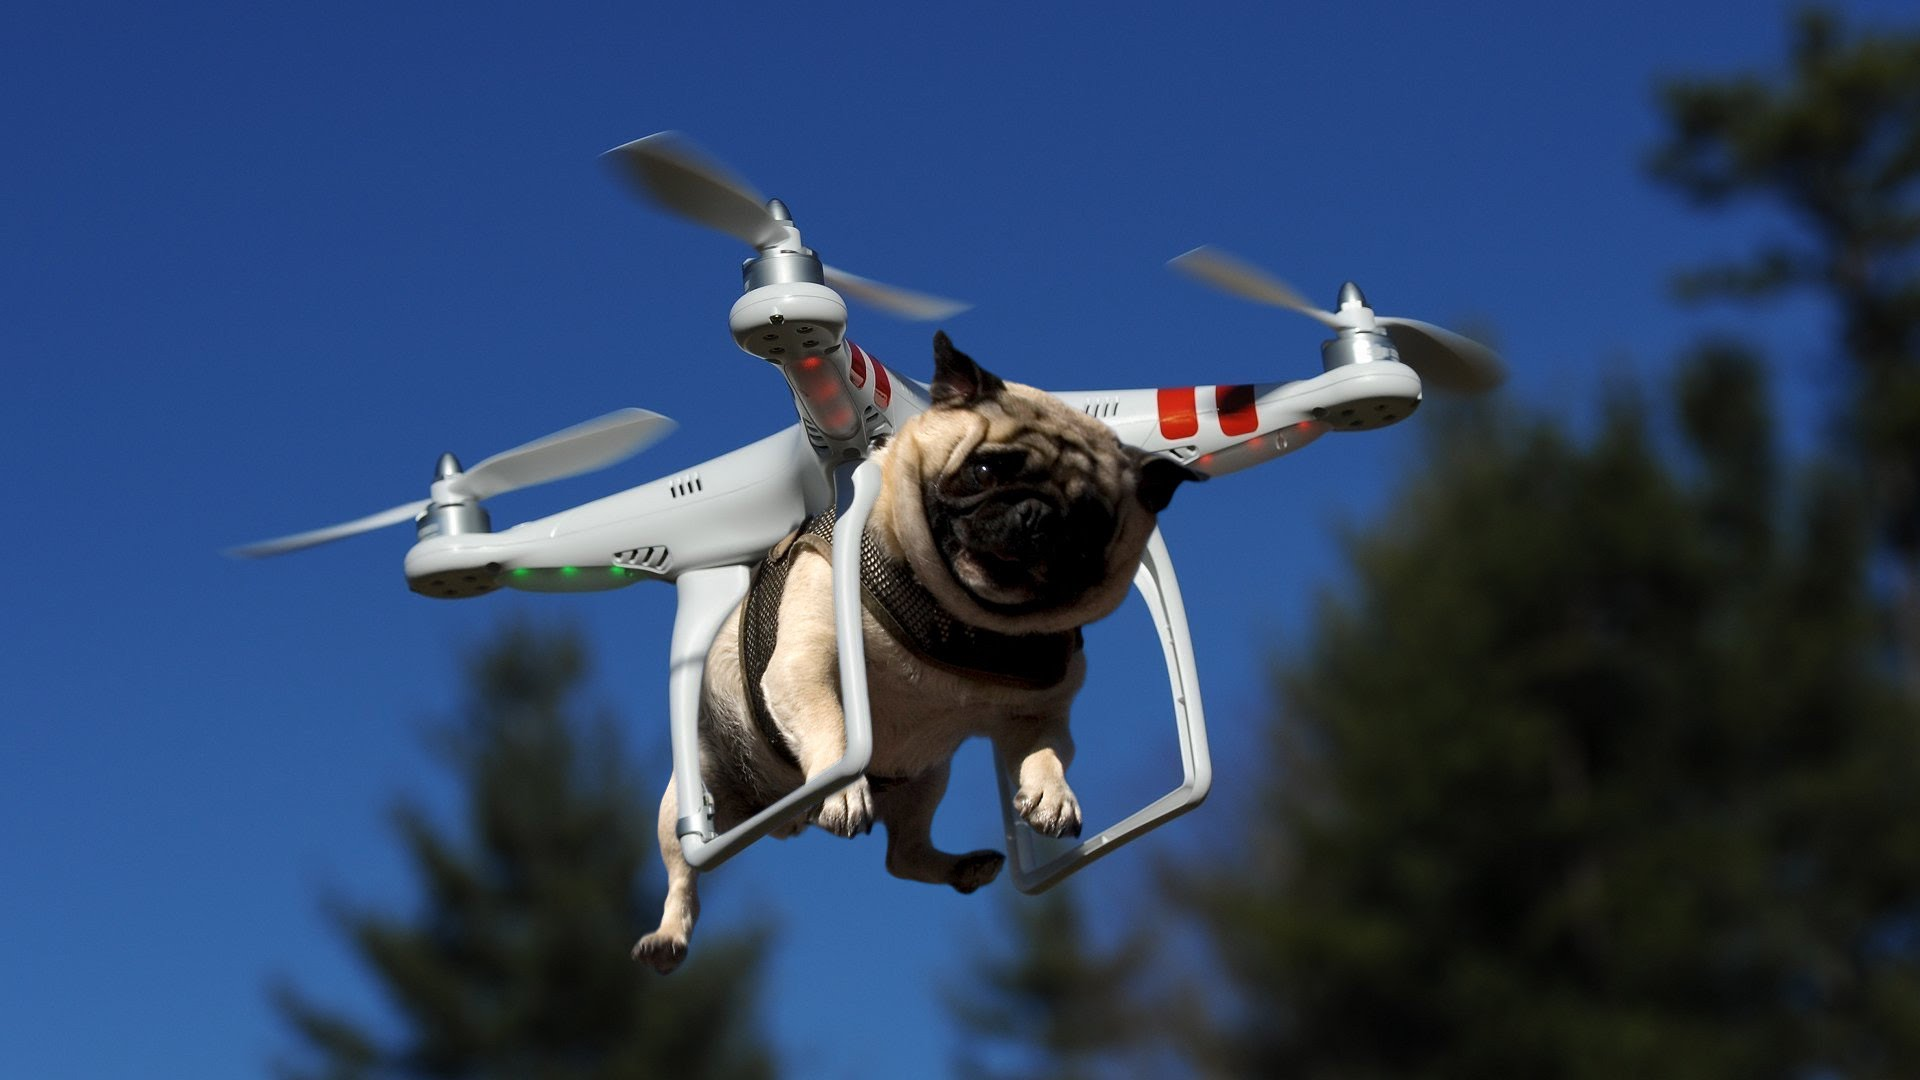
\includegraphics[width=4.9cm]{dog-drone}}
		\hspace{0.3cm}
		\subfigure{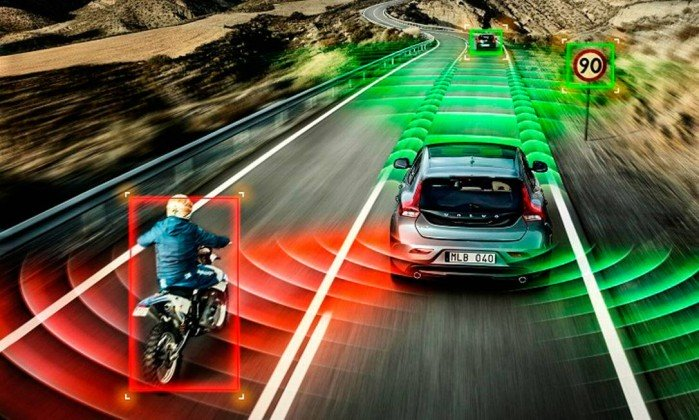
\includegraphics[width=4.7cm]{carros}}
		\\
		\subfigure{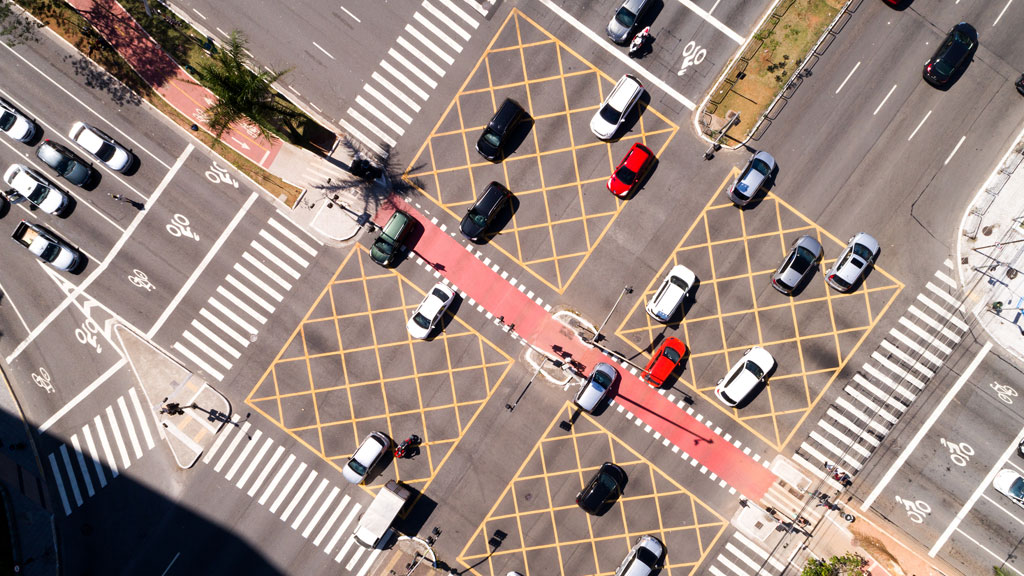
\includegraphics[width=5.5cm]{transito}}
		\subfigure{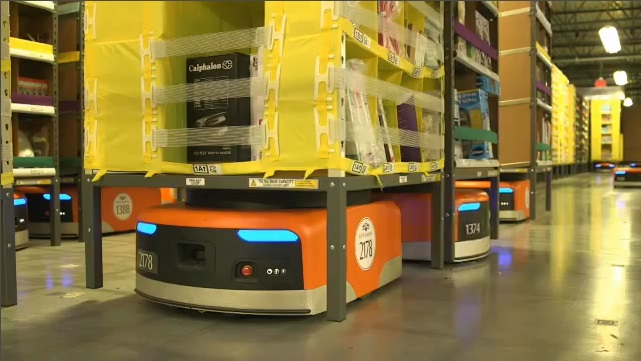
\includegraphics[width=5.5cm]{armazem}}
		
	\end{figure}
\end{frame}

%Slide 1.1
\begin{frame}
\frametitle{\normalsize Savvides, Han e Strivastava, 2001}
\vspace{-0.2cm}
\begin{figure}
	\subfigure{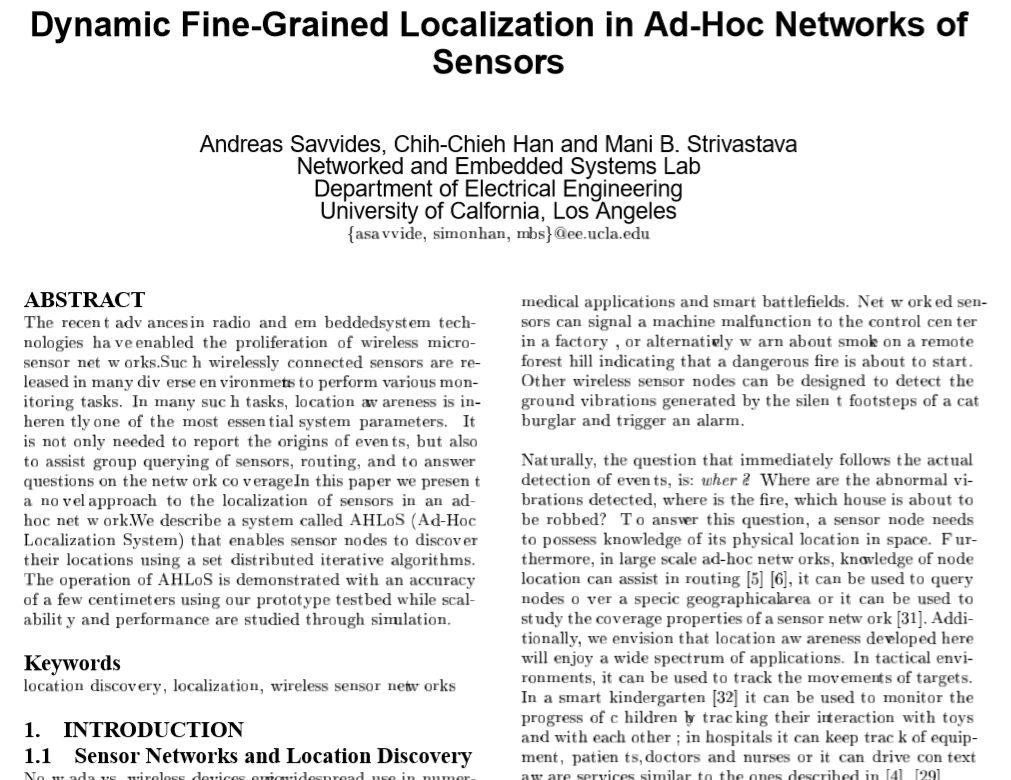
\includegraphics[width=10cm]{savvides}}
\end{figure}
\end{frame}

\section{Redes de sensores e detecção de localização}
%Slide 2
\begin{frame}
	\frametitle{\normalsize Redes de sensores e detecção de localização}
	\begin{flushleft}
		GPS - Sistema de Posicionamento Global
		\begin{itemize}
			\item Utilização dificultada em lugares fechados ou em presença de vegetação densa;
			\item Módulos de GPS possuem consumo energético elevado
			\item GPS é um sistema caro
			\item Baixa precisão
		\end{itemize}
	\end{flushleft}
	\begin{flushright}
		
\includegraphics[scale=0.2]{gps}
	\end{flushright}
\end{frame}


\section{Como modelar um sistema de localização}
%Slide 3
\begin{frame}
	\frametitle{\normalsize Como modelar um sistema de localização}
	\begin{flushleft}
		Questões principais: \\
		\hspace{0.5cm} 1) Como obter os dados?
		\begin{itemize}
			\item Indicador de força do sinal recebido  $ P_{RSSI} = \frac{X}{R^n} $
		\end{itemize}
	
		\begin{figure}
			\subfigure{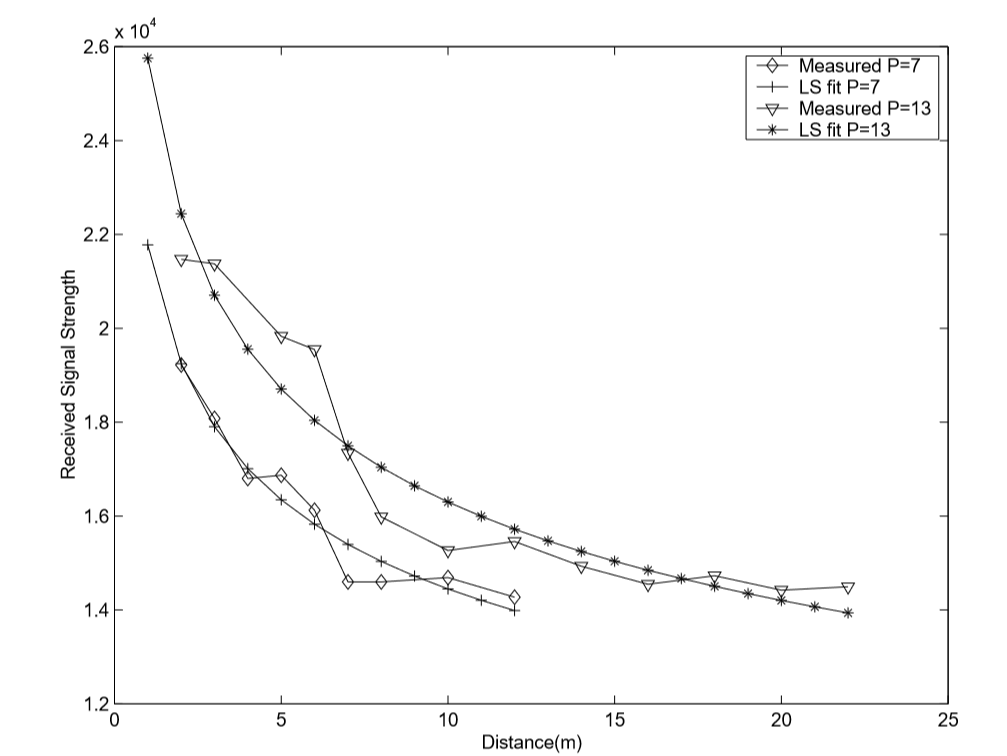
\includegraphics[width=7cm]{RSSI}}
		\end{figure}
	\end{flushleft}
\end{frame}


%Slide 4
\begin{frame}
\frametitle{\normalsize Como modelar um sistema de localização}
\begin{flushleft}
	Questões principais: \\
	\hspace{0.5cm} 1) Como obter os dados?
	\begin{itemize}
		\item Ângulo de chegada
	\end{itemize}
	
	\begin{figure}
		\subfigure{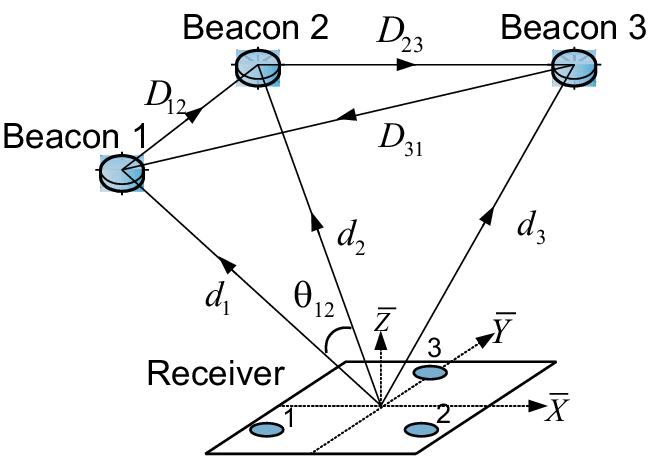
\includegraphics[width=7cm]{AoA}}
	\end{figure}
\end{flushleft}
\end{frame}

%Slide 4
\begin{frame}
\frametitle{\normalsize Como modelar um sistema de localização}
\begin{flushleft}
	Questões principais: \\
	\hspace{0.5cm} 1) Como obter os dados?
	\begin{itemize}
		\item Métodos baseados no tempo (ToA, TDoA)
	\end{itemize}
	
	\begin{figure}
		\subfigure{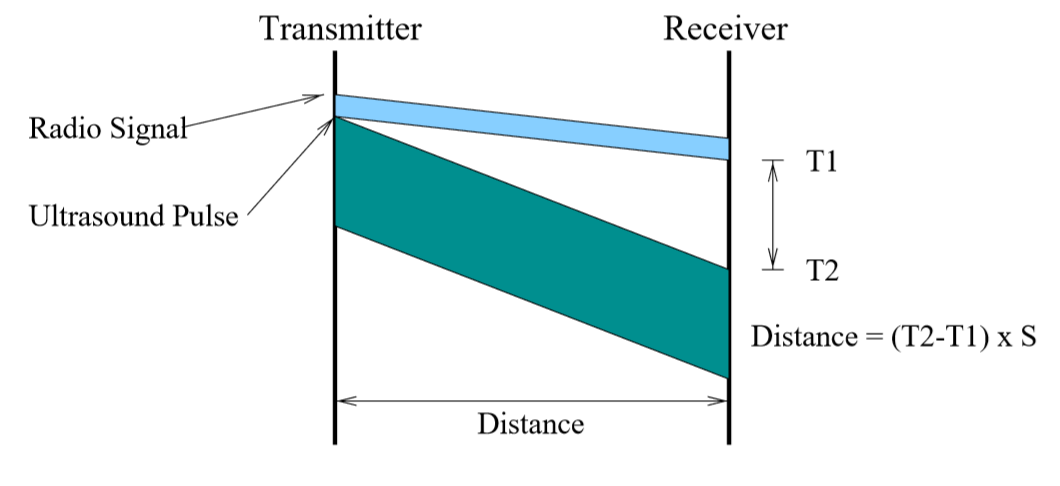
\includegraphics[width=6.5cm]{TDoA}}
		\subfigure{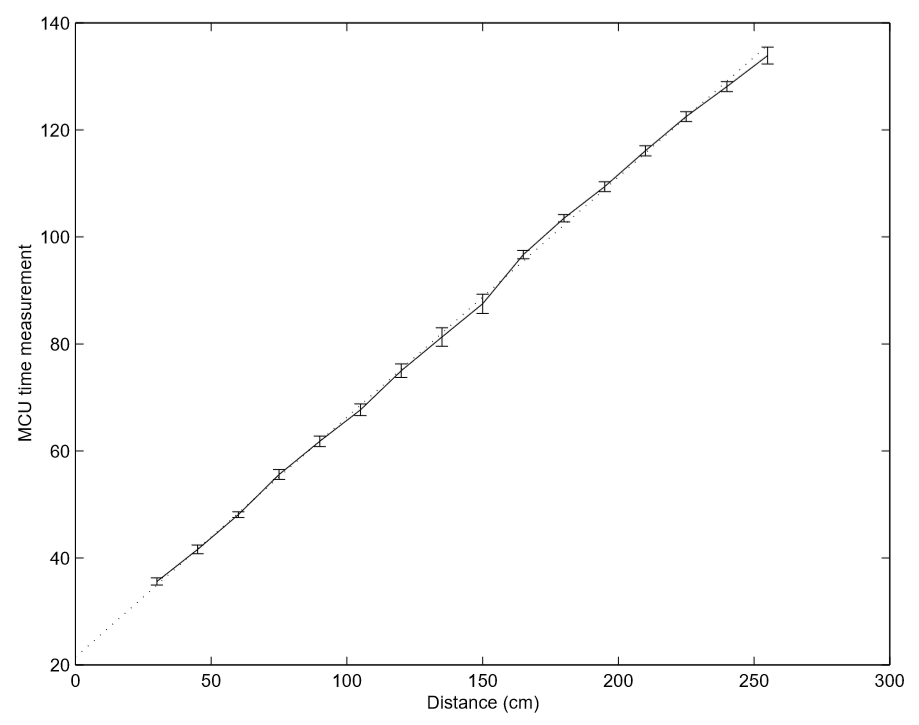
\includegraphics[width=5.0cm]{ToA}}
	\end{figure}
\end{flushleft}
\end{frame}


%Slide 5
\begin{frame}
\frametitle{\normalsize Como modelar um sistema de localização}
\begin{flushleft}
	Questões principais: \\
	\hspace{0.5cm} 2) Como combinar os dados?
	\begin{itemize}
		\item Trilateração hiperbólica
	\end{itemize}
	\vspace{-0.4cm}
	
	\begin{figure}
		\subfigure{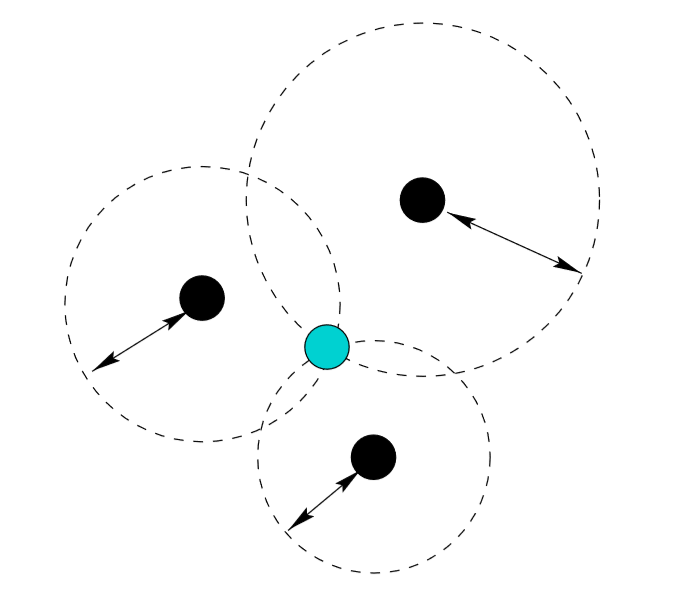
\includegraphics[width=6.5cm]{trilateration}}
		\subfigure{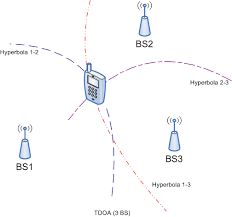
\includegraphics[width=5.0cm]{trilat}}
	\end{figure}
	\vspace{0.4cm}
\end{flushleft}
\end{frame}

%Slide 6
\begin{frame}
\frametitle{\normalsize Como modelar um sistema de localização}
\begin{flushleft}
	Questões principais: \\
	\hspace{0.5cm} 2) Como combinar os dados?
	\begin{itemize}
		\item Triangulação
	\end{itemize}
	
	\begin{figure}
		\subfigure{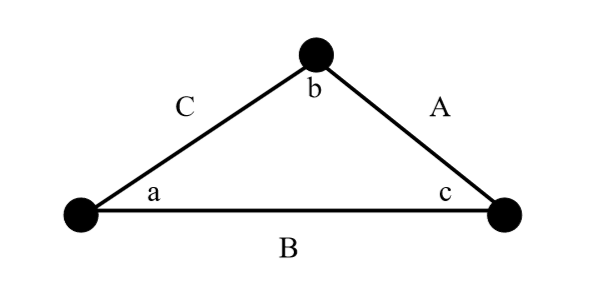
\includegraphics[width=6.0cm]{triangulation}}
		\subfigure{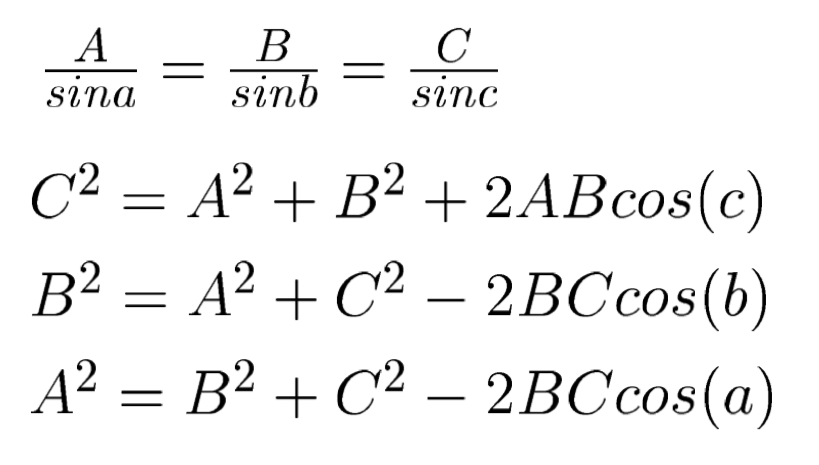
\includegraphics[width=5.5cm]{trigonometrics}}
	\end{figure}
	\vspace{0.4cm}
\end{flushleft}
\end{frame}


%Slide 7
\begin{frame}
\frametitle{\normalsize Como modelar um sistema de localização}
\begin{flushleft}
	Questões principais: \\
	\hspace{0.5cm} 2) Como combinar os dados?
	\begin{itemize}
		\item Multilateração de Máxima Verossimilhança
	\end{itemize}
	\begin{figure}
	\hspace{3.5cm}	\subfigure{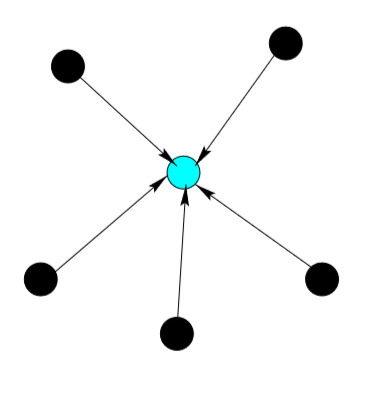
\includegraphics[width=6.0cm]{ml}}
	\end{figure}
	\vspace{0.4cm}
\end{flushleft}
\end{frame}


\section{ML Multilateração - Uma proposta de solução}
%Slide 8
\begin{frame}
\frametitle{\normalsize ML Multilateração}
\begin{flushleft}
	Multilateração Atômica 
	\begin{itemize}
		\item Nós Ancoras - Localização conhecida
		\item Nós Desconhecidos - Possíveis localizações
	\end{itemize}
	
	\begin{figure}
		\subfigure{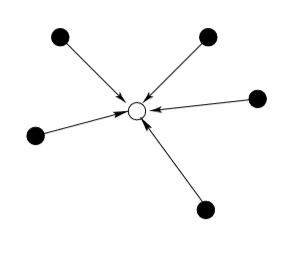
\includegraphics[width=3.0cm]{atomicml}}
		\subfigure{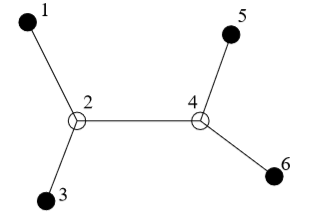
\includegraphics[width=4.0cm]{unknow2}}
		\subfigure{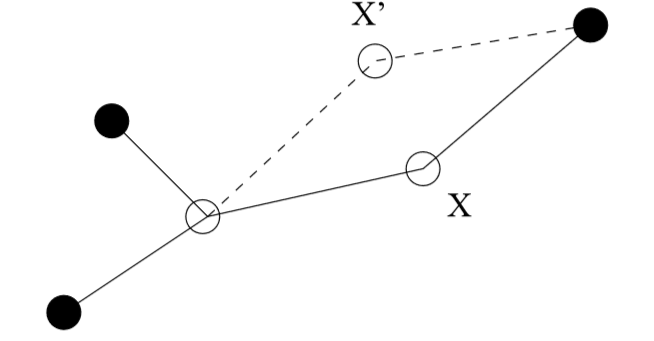
\includegraphics[width=4.0cm]{unknow}}
	\end{figure}
	\vspace{0.4cm}
\end{flushleft}
\end{frame}

%Slide 9
\begin{frame}
\frametitle{\normalsize ML Multilateração}
\begin{flushleft}
	Multilateração Atômica\\
	\begin{figure} 
		\hspace{0.5cm} 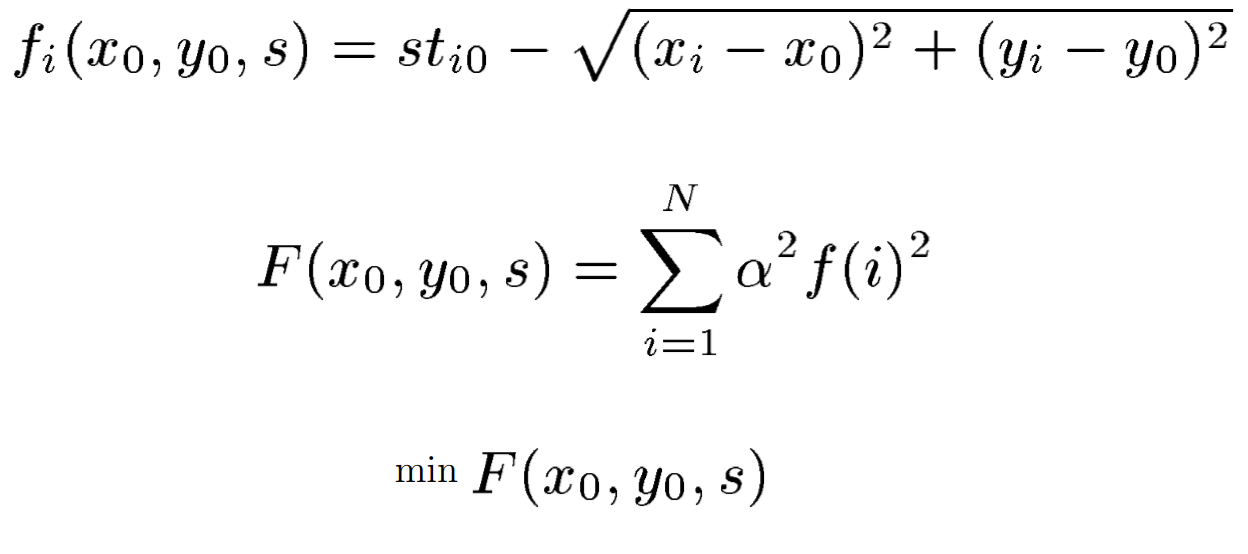
\includegraphics[width=7.0cm]{atomicmleq} \\
	\vspace{0.2cm} \hspace{0.4cm} 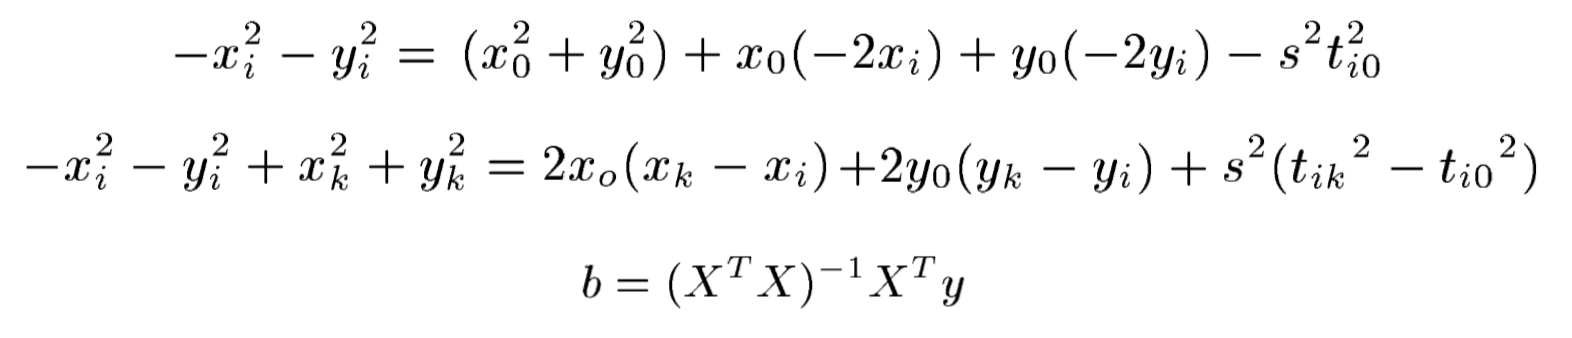
\includegraphics[width=10.0cm]{atomicmleq2}
	 \end{figure}
	\vspace{0.4cm}
\end{flushleft}
\begin{flushright}
	\vspace{-0.6cm}
	Mínimos quadrados
\end{flushright}
\end{frame}

%Slide 10
\begin{frame}
\frametitle{\normalsize ML Multilateração}
\begin{flushleft}
	Multilateração Atômica\\
	\begin{figure} 
		\hspace{0.5cm} 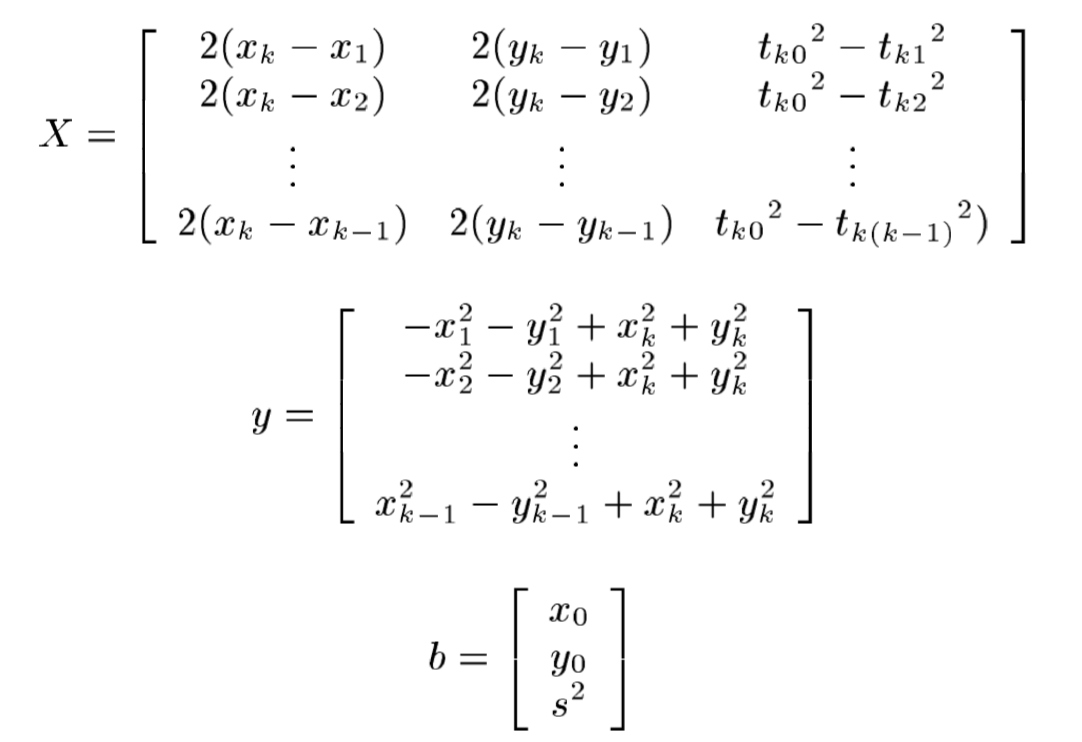
\includegraphics[width=9cm]{atomicmleq3} 
	\end{figure}
	\vspace{0.4cm}
\end{flushleft}
\end{frame}

%Slide 11
\begin{frame}
\frametitle{\normalsize ML Multilateração}
\begin{flushleft}
	\vspace{0.5cm}		
		\begin{center}
			Multilateração atômica só pode ser implantada se o nó desconhecido está dentro do alcance de pelo menos outros três nós ancoras.
		\end{center}
	\vspace{0.4cm}
\end{flushleft}
\end{frame}


%Slide 12
\begin{frame}
\frametitle{\normalsize ML Multilateração}
\begin{flushleft}
	\vspace{-0.2cm}
	Multilateração Interativa\\
	\vspace{0.3cm}
		\textit{boolean} \textit{multilateracaoInterativa}(G)\{
			\\ \hspace{0.5cm} no = nó desconhecido com mais ancoras
			 \\ \hspace{0.5cm} \textbf{while} (no.qtdAncoras $\geq$ 3)\{
			 \\ \hspace{1.5cm} \textit{setAncora}(no)
			 \\ \hspace{1.5cm} no = nó desconhecido com mais ancoras
			\\ \hspace{0.5cm} \}
			\\\}
	\vspace{-1.0cm}
	
	\begin{figure} 
		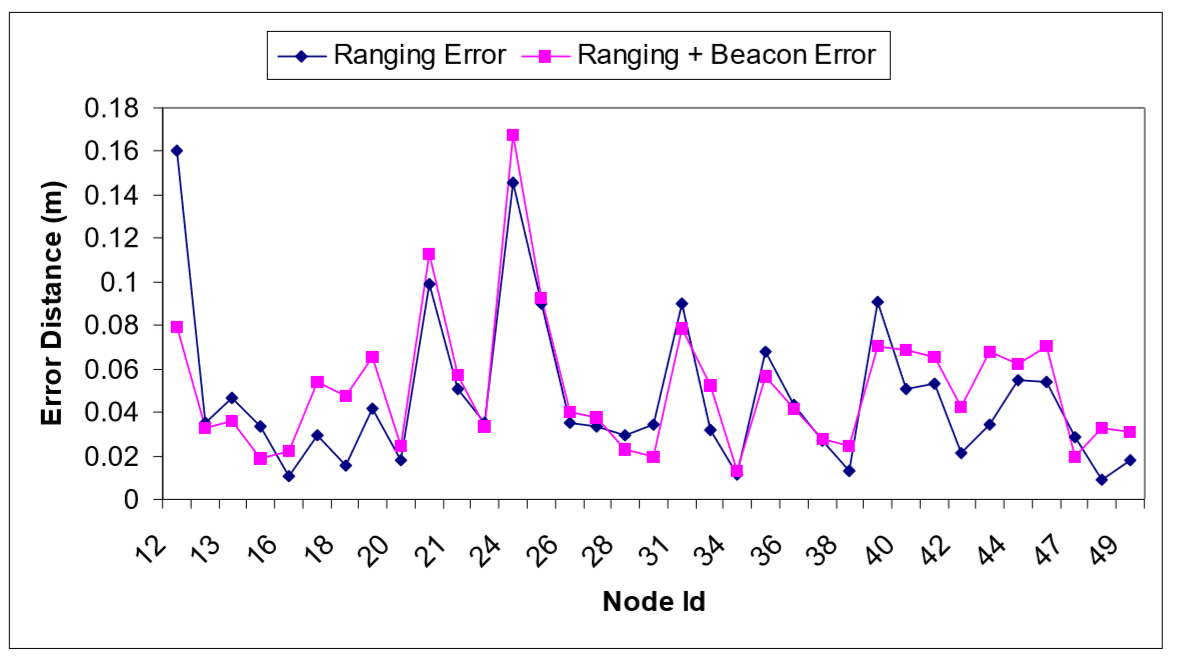
\includegraphics[width=7.5cm]{mli} 
	\end{figure}
\end{flushleft}
\end{frame}

%Slide 13
\begin{frame}
\frametitle{\normalsize ML Multilateração}
\begin{flushleft}
	Multilateração Colaborativa\\
	\vspace{0.2cm}
	\begin{definicao}
		Um nó é dito participante se ele é uma ancora ou se é um desconhecido com pelo menos outros três vizinhos participativos.
	\end{definicao}


	\begin{definicao}
		Par de participação é um par de nós conectados do tipo ancora-desconhecido ou desconhecido-desconhecido onde todos os desconhecidos são participantes.
	\end{definicao}

	\vspace{-0.15cm}
	
	\begin{figure} 
		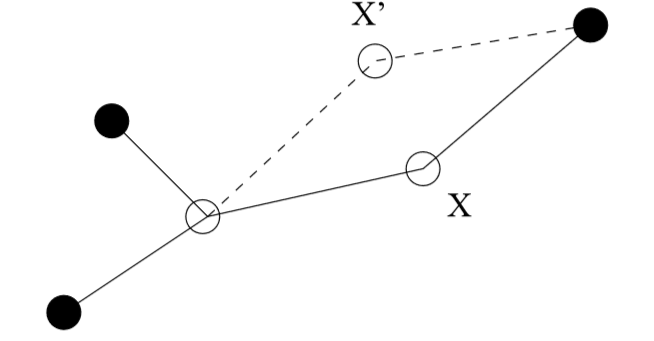
\includegraphics[width=4.5cm]{unknow} 
		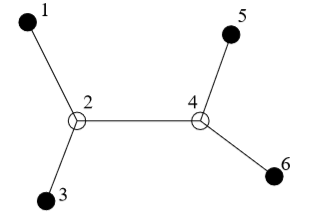
\includegraphics[width=3.5cm]{unknow2} 
	\end{figure}
\end{flushleft}
\end{frame}


%Slide 14
\begin{frame}
\frametitle{\normalsize ML Multilateração}
\begin{flushleft}
	\vspace{-1.5cm}
	Multilateração Colaborativa\\
	\vspace{0.5cm}
	\textit{boolean} \textit{isParticipative}(no, inicial)\{
	\\ \hspace{0.5cm} \textbf{if} (inicial) minimo = 3 else minimo = 2
	\\ \hspace{0.5cm} \textbf{if} (no.qtdAncoras $\geq$ minimo) \textbf{return} true
	\\ \hspace{0.5cm} qtd = no.qtdAncoras
	\\ \hspace{0.5cm} \textbf{foreach} vizinho \textbf{in} no.vizinhos\{
	\\ \hspace{1.5cm} \textbf{if} (\textit{isParticipative}(vizinho, false)) qtd++
	\\ \hspace{1.5cm} \textbf{if} (qtd == minimo) \textbf{return} true
	\\ \hspace{0.5cm}\}
	\\ \hspace{0.5cm} \textbf{return} false
	\\\}
	\vspace{-0.2cm}
	
\end{flushleft}
\end{frame}

%Slide 15
\begin{frame}
\frametitle{\normalsize ML Multilateração}
\begin{flushleft}
	\vspace{-0.3cm}
	Multilateração Colaborativa\\
	\vspace{0.1cm}
	\textit{boolean} \textit{multilateracaoInterativa}(G)\{
	\\ \hspace{0.5cm} no = nó desconhecido com mais ancoras
	\\ \hspace{0.5cm} \textbf{while} (no.qtdAncoras $\geq$ 3)\{
	\\ \hspace{1.5cm} \textit{setAncora}(no)
	\\ \hspace{1.5cm} no = nó desconhecido com mais ancoras
	\\ \hspace{0.5cm} \}
	\\ \hspace{0.5cm} \textbf{while} (isParticipative(no, true))\{
	\\ \hspace{1.5cm} \textit{setAncora}(no)
	\\ \hspace{1.5cm} no = nó desconhecido com mais ancoras
	\\ \hspace{1.5cm} \textbf{while} (no.qtdAncoras $\geq$ 3)\{
	\\ \hspace{2.5cm} \textit{setAncora}(no)
	\\ \hspace{2.5cm} no = nó desconhecido com mais ancoras
	\\ \hspace{1.5cm} \}
	\\ \hspace{0.5cm} \}
	\\\}

\end{flushleft}
\end{frame}

%Slide 16.0
\begin{frame}
\frametitle{\normalsize Introdução Teoria de Grafos}
\begin{flushleft}
	\begin{definicao}
		Um \textbf{grafo} $G = (V,E)$ é definido por dois conjuntos: os vértices $V$ e as arestas $E$, definidas por pares de vértices.
	\end{definicao}
	Perceba, não há restrições para o conjunto $V$.
	\vspace{0.5cm}
	\begin{definicao}
		Um grafo $G = (V,E)$ é dito \textbf{não direcionado} quando o conjunto de arestas $E$ é definido em termos de pares não ordenados de arestas.
	\end{definicao}

	\begin{definicao}
		Em um grafo não-direcionado G, dois vértices u e v são ditos \textbf{conectados} se G contém um caminho de u para v
	\end{definicao}
	
\end{flushleft}
\end{frame}

%Slide 16
\begin{frame}
\frametitle{\normalsize ML Multilateração}
\begin{flushleft}
	\begin{definicao}
		\hspace{0.5cm}Considere um grafo não direcionado conectado $G = (N, E)$ feito de $|N| = n$ nós e um conjunto $E$ de $n - 1$ ou mais arestas. Os nós ancoras são definidos como um conjunto $B$ onde $B \subseteq N$ e o conjunto de nós desconhecidos é $U$ onde $U \subseteq G$. Tem-se a solução do problema encontrando $x_{u}, y_{u} \forall u \in U$ minimizando 
		$$ \sum_{i \in (B \cup U)} (D_{iu} - \sqrt{(x_i - x_u)^2 + (y_i - y_u)^2})^2 $$
		para todos os pares de nós participantes $i$, $u$ onde $i \in B$ ou $i \in U$ e $u \in U$, sujeito a: $x_{i}, y_i$ são conhecidos se $i \in B$, e todo par $i$, $u$ é um par participante.
	\end{definicao}
	
\end{flushleft}
\end{frame}

\section{Um estudo de Complexidade Computacional}
%Slide 17
\begin{frame}
\frametitle{\normalsize Complexidade Computacional}
\begin{flushleft}
Estamos preocupados com um problema de realização.
\vspace{0.1cm}
\\\hspace{0.7cm} Grafos globalmente rígidos
\end{flushleft}
\begin{figure} 
	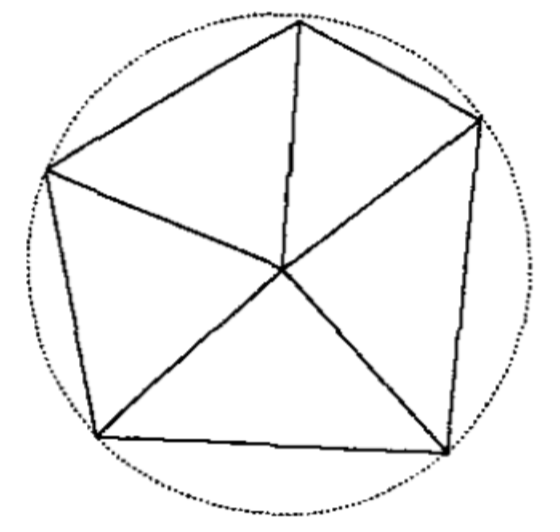
\includegraphics[scale=0.35]{ggr}
\end{figure}
%\begin{definicao}
%	Fidalgo me ajuda a definir melhor, o problema de encontrar a realização de tal partição de conjunto é NP-Difícil.
%\end{definicao}
\end{frame}

%Slide 18
\begin{frame}
\frametitle{\normalsize Complexidade Computacional}
\begin{flushleft}
	Olhando através da otimização global.
	\vspace{0.1cm}
	\\\hspace{0.7cm} Podemos analisar a complexidade sobre um grafo de trilateração $G = (V,E)$ a partir da minimização de 
	$$ \sum_{(i,u) \in E} (D_{iu} - ||i - u||)^2 $$
\end{flushleft}
\begin{definicao}
	Um grafo de trilateração $G = (V,E)$ com configuração realizável é realizável em um número de trilaterações polinomiais.
\end{definicao}
\end{frame}

\section{PGD - Aplicações}
%Slide 19
\begin{frame}
\frametitle{\normalsize Problema de Geometria de Distâncias (PGD)}

\vspace{-1cm}
\begin{definicao}
	Dado um grafo $G = (V, E, d)$, conectado e ponderado nas arestas por $d: E \rightarrow (0, \infty)$, encontre uma função $x: V \rightarrow \mathbb{R}^3$ tal que
	$$\forall \{u, v\} \in E, ||x(u) - x(v)|| = d(u,v).$$
\end{definicao}

\vspace{1cm}
Diz-se que, se o grafo G for completo, tal problema pode ser resolvido com N equações, sendo $N \sim |V|$, possuindo solução em \textbf{tempo linear}.
\end{frame}

%20
\begin{frame}
\frametitle{\normalsize Problema de Geometria de Distâncias (IKP, MDGP, SNL)}
\vspace{-0.5cm}
\begin{figure}
	\subfigure{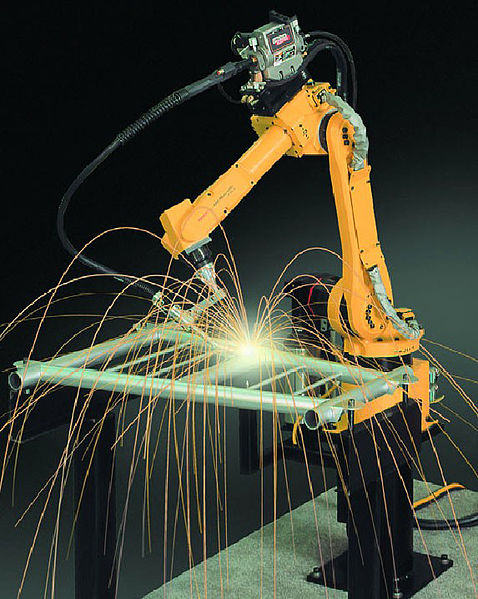
\includegraphics[width=4.0cm]{ikp}}
	\hspace{0.3cm}
	\subfigure{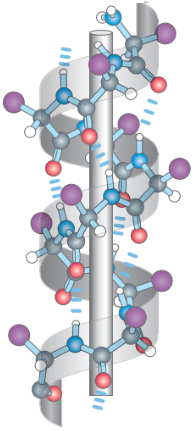
\includegraphics[width=2.5cm]{mdgp}}
	\subfigure{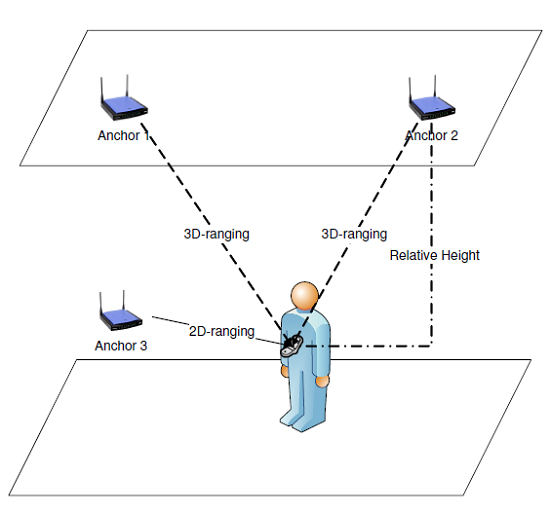
\includegraphics[width=4.5cm]{snl}}
\end{figure}
\vspace{-0.5cm}
\begin{teo}
	\centering
	O PGD é um problema \textbf{NP-Difícil}.
\end{teo}
\end{frame}

%Slide End
\begin{frame}
\centering
\begin{minipage}{0.3\linewidth}
	\begin{flushleft}
		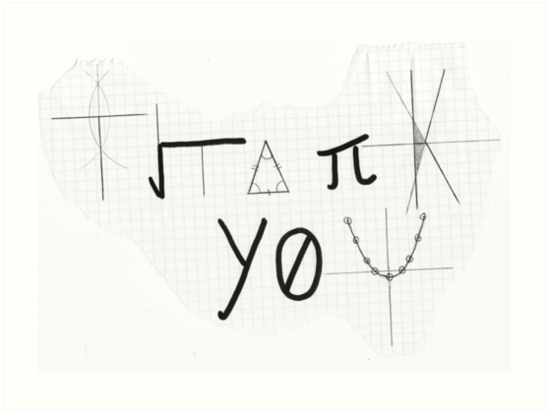
\includegraphics[scale=0.35]{thank}
	\end{flushleft}
\end{minipage}
\hspace{2.5cm}
\begin{minipage}{0.4\linewidth} \centering 
	{\color{blue} \underline{guilherme.philippi@hotmail.com}} \vspace{0.2cm}  \\ UFSC - Blumenau
\end{minipage}
\end{frame}

\end{document}
